\chapter{相关工作}\label{chap:related_work}

本章主要介绍二进制翻译的相关工作,包括软硬协同二进制翻译器和纯软件二进制翻译器。
并对二进制翻译器的性能开销进行分析,发现间接跳转的性能开销以及指令集语义差异是二进制翻译器性能的主要瓶颈。
进而为了解决间接跳转的问题,引出了复杂指令集X86处理器的微码缓存的概念,为微译器的设计提供了设计思路。

\section{软硬协同二进制翻译器}

软硬协同二进制翻译器中一个重要的代表是Transmeta公司开发的软硬协同二进制翻译系统,特别是其Crusoe处理器及代码转换器(CMS),是计算机体系结构和软件技术领域的一项重要创新。
这项技术主要围绕动态二进制翻译(DBT),通过软件层实现对X86架构的全面模拟,使得基于超长指令字(VLIW)的微处理器能够执行X86指令集,从而实现了硬件与软件之间的无缝集成和协同工作。

Transmeta的CMS充当了翻译器和优化器的角色,使得基于非X86的VLIW处理器能够执行X86二进制代码。
CMS层的引入不仅实现了架构间的兼容性,还提供了一个动态优化的执行环境,能够在运行时对代码进行优化,从而提高执行效率和能耗性能\cite{dehnertTransmetaCodeMorphing2003}。

如图\ref{img:transmeta_arch}所示,代码转换器将从程序接收到的X86汇编代码指令翻译成微处理器的本机指令(超长指令字)。
通过这种方式,Crusoe 也可以模拟其他指令集架构,例如Crusoe 也能将字节码翻译为其本机指令集中的指令来执行 Java 字节码。

这种架构有如下特点:
\begin{itemize}
\item 架构兼容性与灵活性:Transmeta的CMS使得原本设计用于执行特定指令集的硬件能够执行广泛的X86指令集,提供了极高的兼容性和灵活性。
\item 动态优化:翻译器不仅在初次执行时翻译代码,还能根据代码的执行特征动态地重新优化代码,以提高运行效率。
\item 异常和中断的处理:CMS设计了独特的机制来处理在动态二进制翻译环境中的异常和中断,确保了系统的稳定性和兼容性\cite{dehnertTransmetaCodeMorphing2003}。
\end{itemize}

\begin{figure}[h]
    \centering
    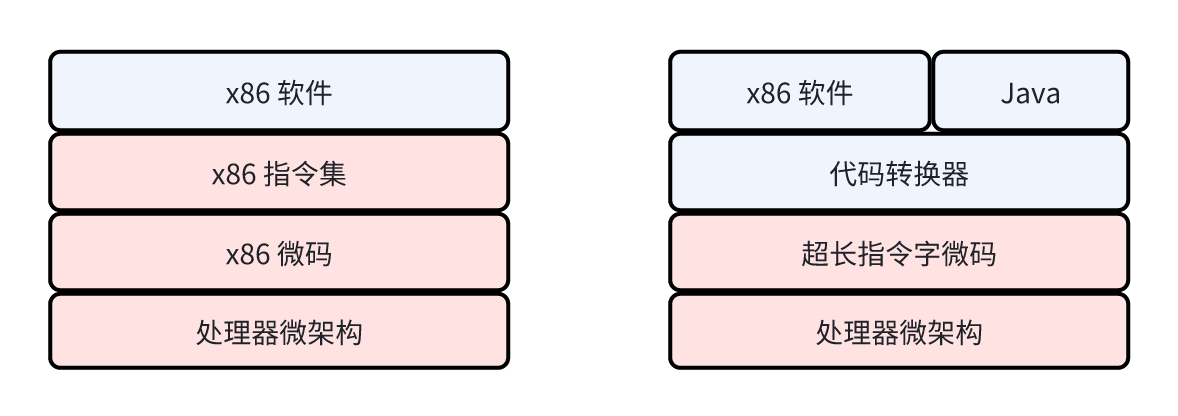
\includegraphics[width=0.8\linewidth]{./feishuImage/transmeta_arch.png}
    \caption{Transmeta架构图,在超长指令字处理器上实现兼容X86的指令集,并支持JAVA程序。}
    \label{img:transmeta_arch}
  \end{figure}


由于目前超标量乱序处理器的硬件乱序调度已经十分成熟,超长指令字设计在通用处理器上的流行度已经减弱,但Transmeta公司在多架构兼容性方面的工作提供了宝贵的经验,成为软硬结合二进制翻译器的重要先驱者。

\section{纯软件二进制翻译器}

在纯软件领域,用户态二进制翻译器扮演着重要的角色。本节主要介绍一款开源的用户态二进制翻译器QEMU,以及一些商用级的用户态二进制翻译器,如苹果公司的Rosetta2、华为公司的ExaGear、龙芯公司的LATX等。

\subsection{QEMU}

QEMU是一个广泛使用的开源虚拟化软件,特别在云计算环境中,它常和KVM一起使用,提供了一种高效的虚拟化解决方案。
QEMU同时支持系统态翻译和用户态翻译,本文主要关注用户态翻译部分,它允许在一个主机操作系统上模拟另一个操作系统的应用程序。

QEMU也同时支持多种架构,包括x86、ARM、RISCV等,使其成为开发跨平台应用程序的理想工具, 也可用于软件开发、测试以及安全研究。
如图\ref{img:qemu_arch},它通过将不同指令集的机器代码翻译成中间语言(IR,Intermediate Representation),再将IR翻译成宿主指令集,实现跨架构的兼容性。
这种设计使得QEMU能够处理多种指令集,为用户提供了一定的灵活性。然而,QEMU的性能仅能达到原生性能的13\%,这主要归因于双层翻译(客户代码翻译到IR,IR翻译到宿主代码)的性能损失。

\begin{figure}[h]
  \centering
  \includegraphics[width=0.6\linewidth]{./image/qemu-IR.pdf}
  \caption{QEMU二进制翻译器架构图,能在宿主指令集机器上运行多种客户程序。}
  \label{img:qemu_arch}
\end{figure}

基于QEMU的优化主要旨在提高其性能和执行效率,特别是在动态二进制翻译(DBT)方面。以下是一些显著的优化实例,包括HQEMU的多线程并行翻译和执行,以及寄存器分配的优化。

HQEMU\cite{Hong2012HQEMUAM}是一个基于QEMU和LLVM构建的多线程和可重定向动态二进制翻译器。这个项目的目标是通过利用多核处理器的并行处理能力来减轻DBT的开销,同时允许更复杂的优化技术的应用。
HQEMU通过在不同的线程上分别运行转换器和动态二进制优化器,从而实现了这一目标。这种方法可以有效地减少DBT对目标应用程序的影响,从而提高整体性能。
在一系列基准测试中,比如SPEC CPU2006,HQEMU在x86到x86-64的模拟中,相比于原始的QEMU性能提高了2.4倍至4倍。
这表明HQEMU仅比原生执行慢2.5倍至2.1倍,而原始QEMU则慢了6倍至8.4倍。

在动态二进制翻译中,寄存器分配是提高翻译代码执行效率的关键。原始的QEMU在许多宿主机上将所有目标寄存器映射到内存,并仅将少数临时变量存储在宿主寄存器中。
这种方法并没有考虑相邻指令之间的依赖关系,导致即使在执行前一个指令时已经将一个客户寄存器的值加载到临时变量中,执行下一个指令时也需要再次从内存中重新加载该值。
为了解决这个问题,\cite{Hong2012HQEMUAM}提出了一个优化方法,通过消除这些不必要的操作来提高翻译速度。
这种方法在两个或更多相邻指令执行中有效利用了临时变量,从而减少了对内存的不必要访问。通过这种优化,基准测试显示可以实现10\%到20\%的速度提升。

尽管以上优化示例展示了通过改进QEMU的翻译过程和内部机制,可以提升QEMU的效率和性能,但是改进后的性能仅相当于原生性能的一小部分,这在一些对性能要求较高的应用场景下显得不够可用。



\subsection{Rosetta2}

Rosetta2 代表了苹果公司在其Mac计算机上实现x86到ARM指令集转换的先进技术。通过支持即时编译(JIT)和预先编译(AOT)两种模式,
Rosetta2 允许在运行时动态翻译指令或在软件安装时直接翻译成ARM指令。
这种技术的实现关注于用户态指令的翻译,而不包括特权指令、虚拟化扩展等复杂的x86指令集部分。此外,Rosetta2 主要针对64位的x86\_64指令集进行翻译,以适配苹果M1等64位处理器的架构。

Rosetta2 的核心目标是保证MacOS上的软件能够在ARM架构下运行,这要求对系统调用进行转换,以匹配基于ARM的MacOS版本。
由于x86和ARM指令集都采用小端法(little-endian),这简化了指令翻译过程,避免了复杂的字节序反转操作。
这一点与苹果过去从PowerPC(大端法,big-endian)切换到x86的过程不同,后者在转换时面临更多的挑战。

然而,x86(强内存序)与ARM(弱内存序)在内存一致性模型上的差异可能导致多线程软件运行结果出现差异,这是模拟x86的一个主要挑战\cite{Risotto}。
苹果通过在芯片内部额外实现一个Intel版本的强内存TSO模型,并通过后门开关在运行Rosetta2时切换到该内存模型,解决了这一问题。这种设计可能是Rosetta2性能优异的关键因素。

综上所述,Rosetta2通过精巧的技术和优化,实现了在苹果的ARM架构处理器上运行原本为x86架构设计的MacOS软件的能力。
这不仅展示了苹果在软硬件兼容性方面的创新能力,也为跨架构软件运行提供了宝贵的技术参考。

\subsection{ExaGear}

ExaGear是华为公司开发的动态二进制翻译软件,专为在基于ARM的服务器上运行而设计。该软件能够实时将x86架构的指令转换为ARM架构的指令,从而允许原本只能在x86平台上运行的应用程序无需任何修改即可在ARM平台上执行。
这种技术的开发是响应了日益增长的对ARM服务器的兴趣,这些服务器以其能效比优势在数据中心环境中越来越受欢迎。

ExaGear通过修改Linux的binfmt\_misc组件,使得系统能够识别并使用ExaGear作为x86应用程序的解析器,实现了在安装过程中的高效集成。
ExaGear主要包括两个关键组件:指令翻译引擎和x86运行环境。指令翻译引擎充当x86应用程序与ARM架构服务器之间的中间件,实现了在x86应用程序启动时的实时翻译功能。
这一过程对用户完全透明,确保了用户体验的一致性。x86运行环境为x86应用程序提供了必要的标准库、实用程序和配置文件,构建了一个完整的运行时环境。
这一环境通过模拟x86架构下的操作系统环境,确保了应用程序能够在ARM服务器上无缝运行,同时保持了运行效率和稳定性。

这种动态指令翻译技术的应用不仅降低了将x86应用迁移到ARM服务器的成本和复杂性,也为软件的跨平台兼容性和服务器架构的多样性提供了强有力的支持。
随着ARM架构在服务器市场的持续增长,ExaGear及类似技术的开发为实现更高效、更经济的计算资源利用开辟了新的路径。


\subsection{LATX}

龙芯二进制翻译器(LATX)是龙芯公司开发的一款动态二进制翻译软件,用于在龙芯处理器(LoongArch架构)上运行x86架构的应用程序。
结合LATX和Wine\cite{amstadt1994wine}(一 个 操 作 系 统 API翻译软件,它可以用Linux的系统调用来模拟实现Windows的系统调用,从而实现在Linux/ x86上运行Windows/x86的应用程序),
用户可以在龙芯处理器上运行大量的x86应用程序,包括Windows应用程序,例如微信、WPS、部分游戏等。

龙芯早期使用MIPS指令集,并添加了便于X86和ARM二进制翻译的一系列自定义指令集,例如对X86 EFLAGS的支持、对X87浮点指令的支持、非对齐访存的支持等,形成了LoongISA\cite{LoongISA}。
但由于MIPS中用户定义指令(UDI)槽位有限,导致了LoongISA的指令集扩展受限,所以在2020年龙芯公司发布了全新的、自主可控的、支持更多指令集扩展的LoongArch架构\cite{LoongArch2023}。
并从3A5000开始,龙芯处理器开始支持LoongArch架构,并配套使用LATX进行x86应用程序的翻译。
LoongArch指令集中同样增加了对二进制翻译的扩展指令集,称为LBT(Loongson Binary Translation)指令集,用于支持x86、ARM、MIPS的二进制翻译。
LBT扩展指令集与LATX软件配合使用,可以实现更高效的二进制翻译,提高了龙芯处理器的软件兼容性。


\section{纯软件二进制翻译的性能开销分析}

其他常用的商用级用户级二进制翻译器,参见表\ref{tab:BTs},例如苹果公司的Rosetta2(67.2\%)、华为公司的ExaGear(72.7\%)、龙芯公司的LATX(60\%)等,性能上仍然无法接近原生性能。
这些二进制翻译器采用一对一指令的翻译方式,即把一种指令集直接翻译到另一种指令集上(但一条客户指令可能翻译成多条宿主指令,产生指令膨胀,导致性能下降)。
它们虽然在理论上支持多架构翻译,但实际上需要投入较大的工程量,也可能造成性能下降。

\begin{table}[]
\centering
\caption{主流二进制翻译器}
\label{tab:BTs}
  \begin{tabular}{llll}
  \rowcolor[HTML]{FBE5D6} 
  二进制翻译器    & 公司   & 客户平台           & 宿主平台           \\
  ExaGear   & 华为   & X86            & ARM            \\
  Rosetta2  & 苹果   & X86            & ARM            \\
  LoongArch & 龙芯   & X86            & LoongArch      \\
  QEMU      & 开源项目 & X86,ARM,RISCV等 & X86,ARM,RISCV等
  \end{tabular}
  \end{table}

\begin{figure}[h]
  \centering
  \rotatebox{90}{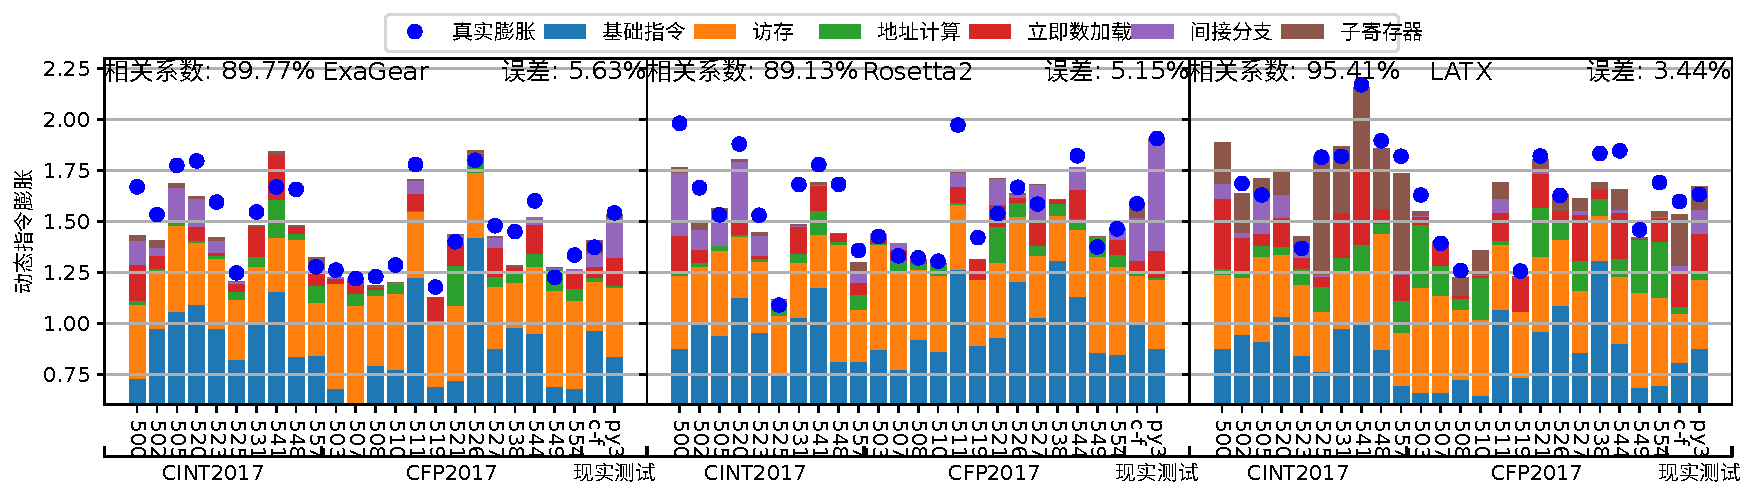
\includegraphics[width=\textheight,height=\textwidth,keepaspectratio]{./plot/insts_inflt_breakdown_2017.pdf}}
  \caption{各个二进制翻译器在运行SPEC2017的指令膨胀来源分析图。}
  \label{img:insts_inflt_breakdown_2017}
\end{figure}

根据我们之前完成的一项工作,使用指令膨胀率来分析二进制翻译器的性能开销。指令膨胀率是指,每条客户指令平均翻译出的宿主指令数,是一个大于1的小数,计算方式为$\mbox{总体膨胀} = \mbox{生成的宿主指令数} / \mbox{客户指令数}$(这里用的是动态运行指令数)。指令膨胀率越高,翻译后的程序要执行的指令数越多,执行时间越长,性能越低。即便多发射处理器能在单拍内执行多条指令,缓解更多指令带来的性能开销,但根据我们的测试数据,指令膨胀率和性能下降值是保持正相关的。如图\ref{img:insts_inflt_breakdown_2017},我们主要把开销分成了5类:

%latex 使用1. 2. 3. 来编号
\begin{enumerate}
  \item \textbf{指令集间操作码差异:} 不同指令集的操作码差异引起Eflags计算等操作的额外指令翻译,增加了指令膨胀率。此外LoongArch对于子寄存器默认符号扩展,X86/ARM默认零扩展。对应图\ref{img:insts_inflt_breakdown_2017}中\textcolor{brown}{棕色}部分。
  
  \item \textbf{操作数据模式不同:} 复杂指令集(如X86)可以直接访问内存,而其他精简指令集只能操作寄存器,导致操作数模式不同。对应图\ref{img:insts_inflt_breakdown_2017}中\textcolor{orange}{橙色}部分。
  
  \item \textbf{地址计算不同:} 复杂地址计算方式(如X86)与其他指令集的简单计算方式导致在翻译时需要额外指令。例如X86计算地址$addr = base + index * scale +disp$; 其他的大多为$addr = base + offset$。 对应图\ref{img:insts_inflt_breakdown_2017}中\textcolor{green}{绿色}部分。
  
  \item \textbf{立即数加载:} X86支持编码64位立即数和32位地址偏移,而其他指令集编码空间有限,导致立即数加载的语义不同,需要额外的访存指令或者是多条立即数加载指令。对应图\ref{img:insts_inflt_breakdown_2017}中\textcolor{red}{红色}部分。
  
  \item \textbf{间接跳转:} 客户指令地址到宿主指令地址是非线性的,而间接跳转的目标地址在运行时才能知道,需要查询间接跳转哈希表,导致性能开销。对应图\ref{img:insts_inflt_breakdown_2017}中\textcolor{purple}{紫色}部分。
  
\end{enumerate}

以上这5类主要开销很难通过软件优化来解决,需要借助硬件辅助的方式来解决。

为了消除软件二进制翻译器的性能开销,特别是在处理指令集语义差异方面的挑战,本文采用了硬件辅助的策略。其中,一些关键的工作包括:

1. 融合微码以缩小指令集语义差距: 针对指令集间操作码差异、操作数据模式不同以及地址计算不同等问题,我们尝试通过融合微码的方式,减小不同指令集之间的语义差距,从而降低翻译的开销。

2. 微码缓存的思路应用: 针对立即数加载和间接跳转的性能开销,我们借鉴了X86微码缓存的思想,将立即数放入微码缓存行中直接加载,用微码缓存直接查询非线性的地址空间映射,消除这两类开销。

接下来,将介绍与X86微码缓存相关的工作,探讨如何借助硬件辅助手段进一步优化软件二进制翻译器的性能。


% \section{X86 微码缓存的相关工作}
\section{复杂指令集处理器}

X86 微码缓存是为了在 X86 CPU 后端实现超标量乱序执行并降低译码功耗而引入的关键组件\cite{solomonMicrooperationCachePower2001},如图\ref{img:front_end_ucache}。以下是关于 X86 微码缓存的主要工作和设计特点:

\begin{figure}[h]
  \centering
  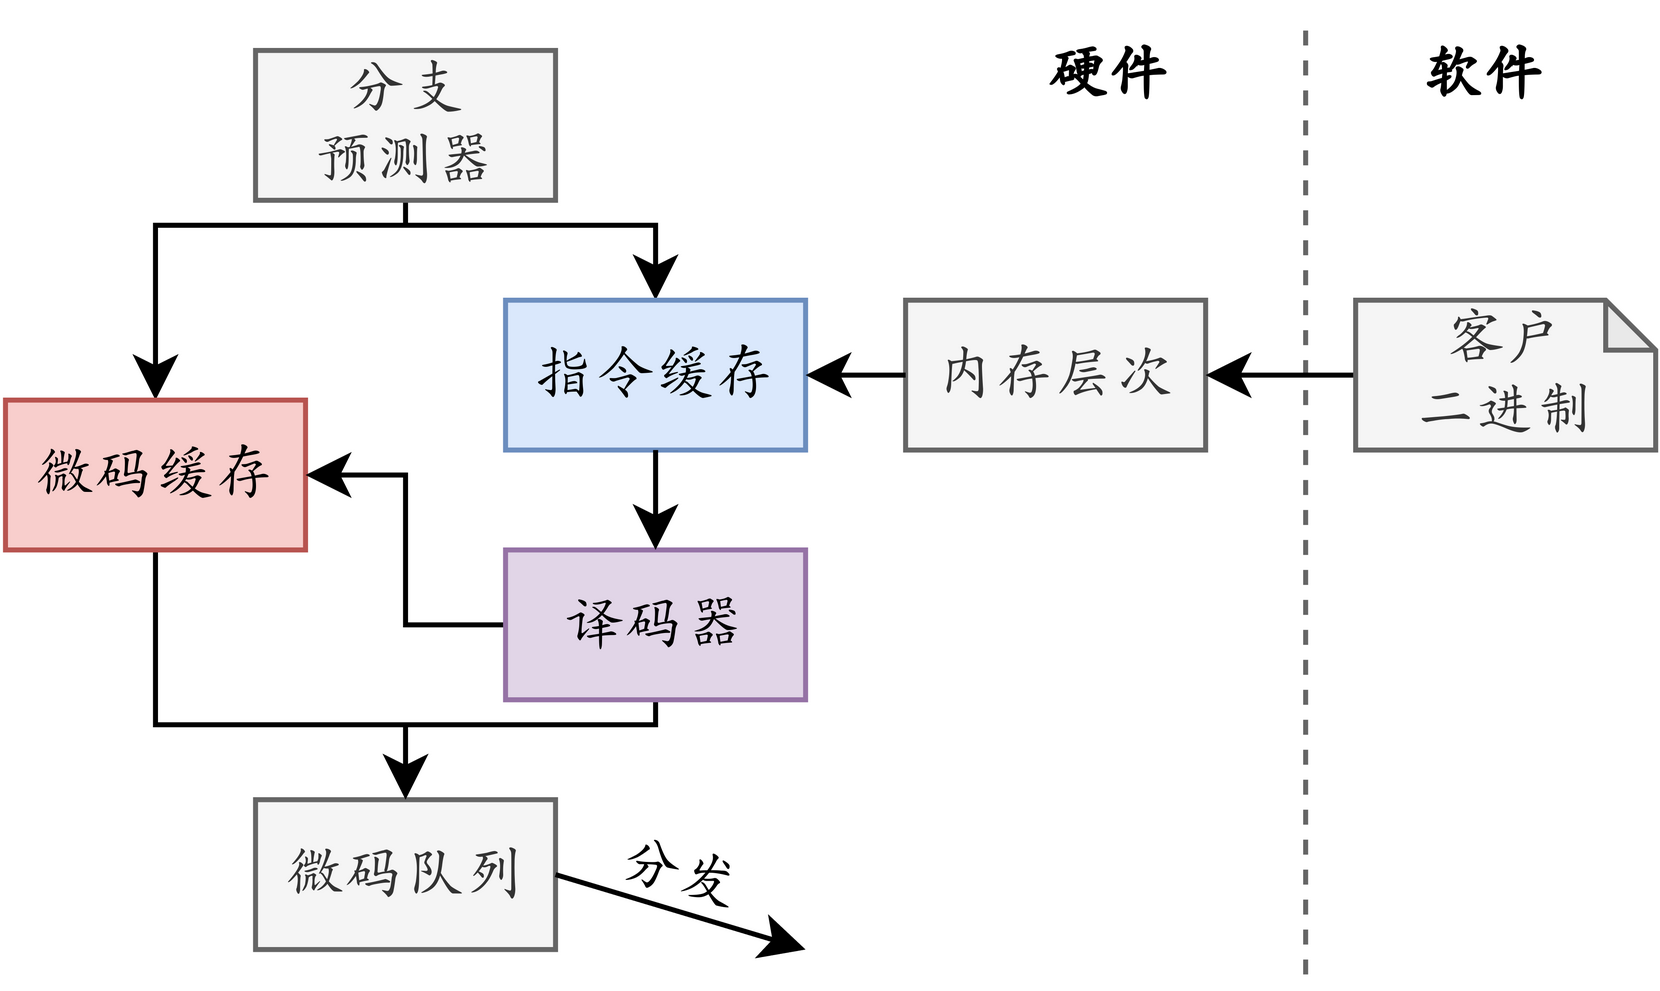
\includegraphics[width=0.8\linewidth]{./image/front_end_ucache.pdf}
  \caption{X86处理器前端架构图,包括指令缓存和微码缓存}
  \label{img:front_end_ucache}
\end{figure}

\begin{figure}[h]
  \centering
  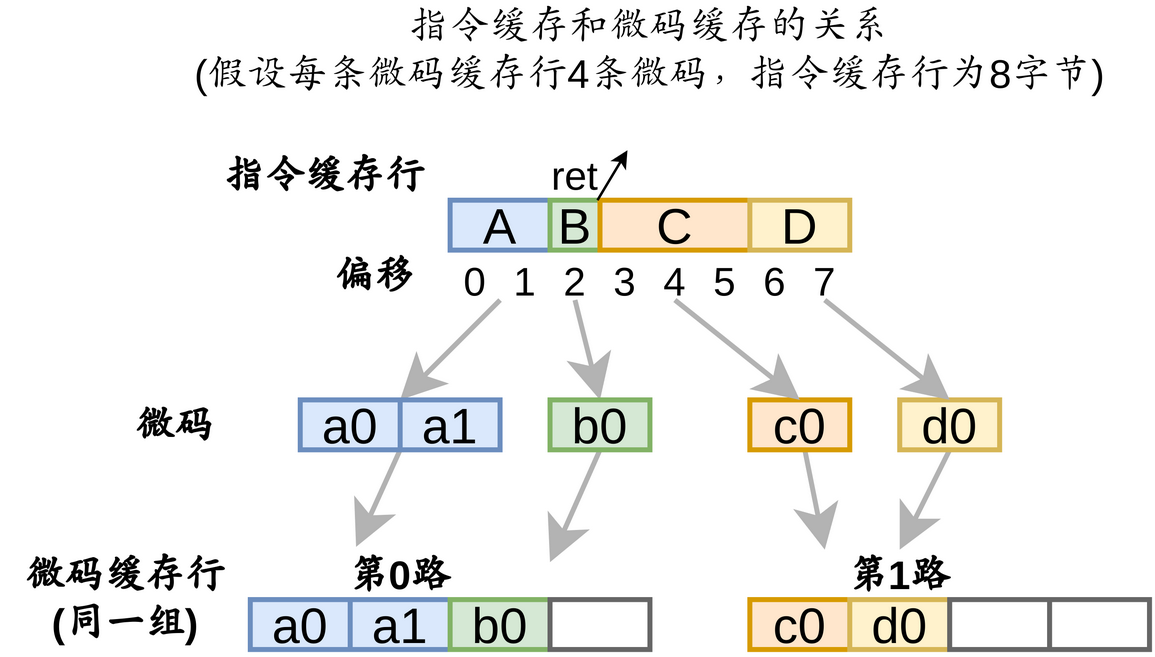
\includegraphics[width=0.8\linewidth]{./image/IC-to-UC.pdf}
  \caption{指令缓存和微码缓存关系}
  \label{img:IC_to_UC}
\end{figure}

1. \textbf{微码与超标量乱序执行的关系:}

   - 为了实现超标量乱序执行,X86 CPU 后端需要将复杂指令译码为简单指令,即微码。

   - 微码的引入简化了指令集的关系,使得 CPU 在后端能够更高效地执行。

2. \textbf{微码缓存的引入:}

- 为了降低译码能耗、提高性能,研究者们引入了微码缓存,用于存储已经译码过的微码。

- 微码缓存的设计目的是减少译码的重复计算,从而提高整体指令执行效率。

3. \textbf{查询与缓存机制:}
  
- 在前端译码阶段,系统首先查询微码缓存,检查是否已经缓存了当前指令的微码。

- 如果微码已经在缓存中,CPU 就直接读取微码并发射到后端执行。

- 如果微码未缓存,系统则从指令缓存中取得指令,进行译码,并将译码结果存入微码缓存中,见图\ref{img:IC_to_UC},注意一个指令缓存行可能生成多个微码缓存行。

4. \textbf{缓存组织形式:}

- 微码缓存的组织形式与指令缓存有所区别。它以第一条指令的程序计数器(PC)作为索引,来索引整行的微码。

- 当遇到控制流指令时,微码缓存会截断这一行,确保每个缓存行只包含一个基本块的微码,参考图\ref{img:IC_to_UC}中的ret指令。

- 微码行中除了存入微码外,还会在最后存储立即数,见图\ref{img:ucache_line},这是由于X86是变长指令集,微码是定长指令集,遇到长立即数时候就会放在微码行最后。

X86 微码缓存的引入和优化为 X86 架构的超标量乱序执行提供了重要支持,使得 CPU 在执行 X86 指令集时能够更加高效地利用硬件资源,提高整体性能。

\begin{figure}[h]
  \centering
  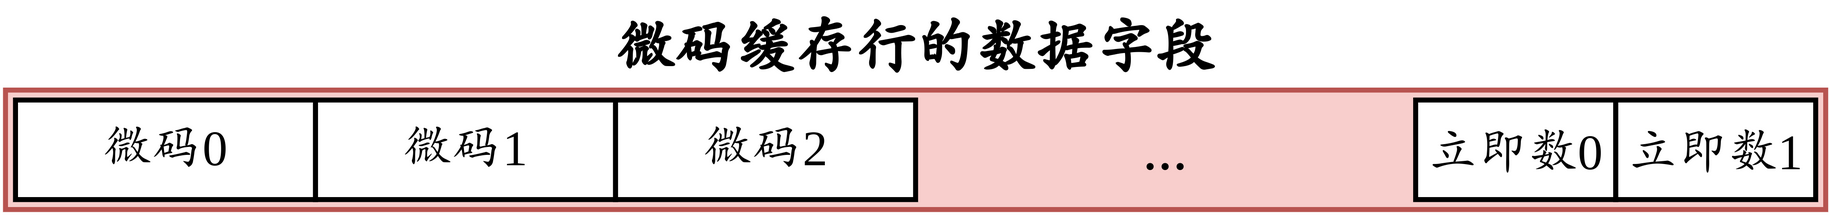
\includegraphics[width=0.8\linewidth]{./image/ucache_line.pdf}
  \caption{微码缓存一行的内容}
  \label{img:ucache_line}
\end{figure}
